\newpage

%\section[Тестирование]{\large \centering Тестирование}
%\hspace{\parindent} 2 блока тестов - тесты MACSE и синтетические тесты для оценки скорости

%\subsection[Оценка качества полученного выравнивания]{\large Оценка качества полученного выравнивания}
%\hspace{\parindent} Примеры из контача

\section[Оценка производительности]{\large \centering Оценка производительности}
\hspace{\parindent} Производительность разработанного алгоритма против существующей программы парного выравнивания MACSE оценивалась на группах синтетических тестов --- наборы созданных случайных последовательностей нуклеотидов заданной длины. Тестирование происходило на машине с процессором Intel Xeon E5645 под управлением ОС Linux Debian 7 (wheezy). Результаты тестирования представлены в таблице~\ref{tabular:results}, гистограмме (рисунок~\ref{ris:gist}) и на точечном графике (рисунок~\ref{ris:3D}).\\
\indent При тестировании были рассмотрены различные сборки разработанной программы: был использован компилятор intel icpc с различными флагами оптимизации и компилятор gcc с флагом -O3. Из графиков и таблицы хорошо видно серьезное замедление времени выполнения на больших тестах для обоих алгоритмов. Сложность полученного решения отличается от MACSE только на константу, тем не менее был получен существенный прирост производительности.

\begin{figure}[h]
	\center{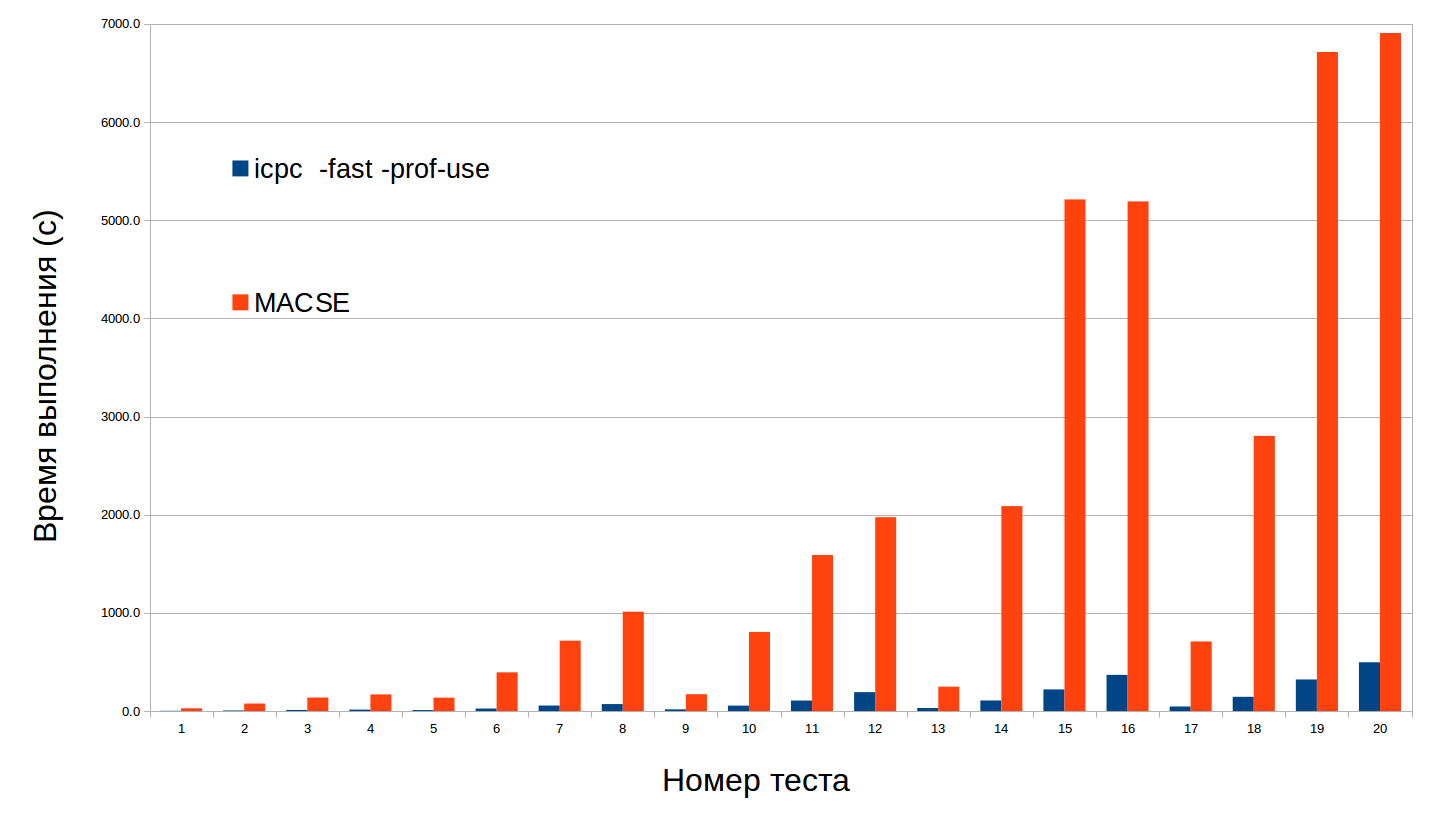
\includegraphics[width=0.65\linewidth]{gist.png}}
	\caption{Время выполнения тестов разработанного алгоритма и MACSE}
	\label{ris:gist}
\end{figure}
\begin{figure}[h]
	\center{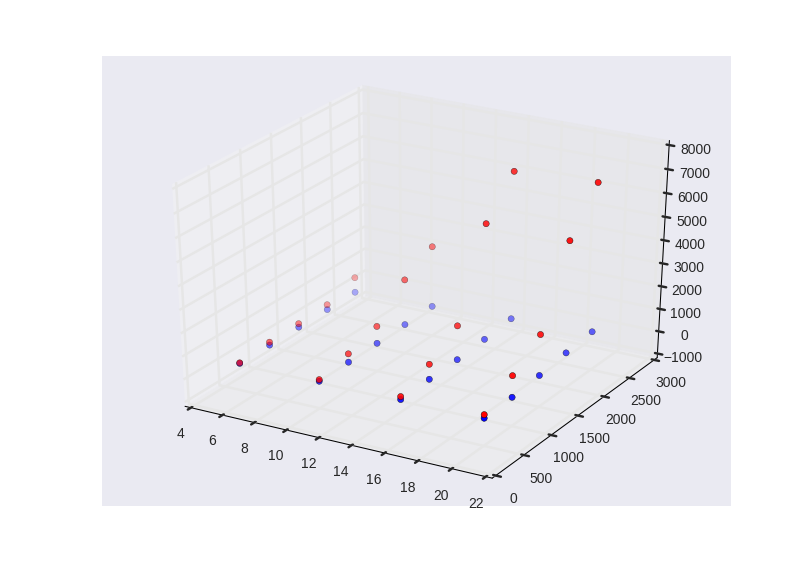
\includegraphics[width=0.65\linewidth]{3D.png}}
	\caption{График роста времени выполнения при увеличении объема входных данных}
	\label{ris:3D}
\end{figure}

\begin{landscape}
\begin{table}[htbp]
\caption{Результаты тестирования}
\begin{longtable}{|*{2}{p{3.5cm}|}*{2}{p{1.8cm}|}*{3}{p{2.8cm}|}*{2}{p{1.8cm}|}}
\hline
\multicolumn{ 1}{|p{3.5cm}|}{Длина поледовательностей} & \multicolumn{ 1}{p{3.5cm}|}{Количество последовательностей} & \multicolumn{ 7}{p{15.6cm}|}{Время выполнения (с)} \\ \cline{ 3- 9}
\multicolumn{ 1}{|p{3.5cm}|}{} & \multicolumn{ 1}{p{3.5cm}|}{} & \multicolumn{ 6}{p{10.8cm}|}{Опции компиляции } & \multicolumn{ 1}{p{1.8cm}|}{MACSE} \\ \cline{ 3- 8}
\multicolumn{ 1}{|p{3.5cm}|}{} & \multicolumn{ 1}{p{3.5cm}|}{} & \multicolumn{1}{p{1.8cm}|}{icpc -O0} & \multicolumn{1}{p{1.8cm}|}{icpc -fast} & \multicolumn{1}{p{1.8cm}|}{icpc  -fast -prof-use} & \multicolumn{1}{p{1.8cm}|}{icpc -fast -parallel} & \multicolumn{1}{p{1.8cm}|}{icpc -fast -prof-use -parallel} & \multicolumn{1}{p{1.8cm}|}{gcc -O3} & \multicolumn{ 1}{p{1.8cm}|}{} \\ \hline
500 & 5 & 11.857 & 2.364 & 2.256 & 2.344 & 2.18 & 2.832 & 27.294 \\ \hline
500 & 10 & 40.171 & 6.724 & 6.096 & 7.196 & 6.06 & 7.748 & 76.309 \\ \hline
500 & 15 & 75.969 & 12.493 & 11.409 & 11.997 & 11.097 & 14.017 & 137.789 \\ \hline
500 & 20 & 114.995 & 18.697 & 14.969 & 16.029 & 15.713 & 18.473 & 169.339 \\ \hline
1000 & 5 & 48.759 & 9.093 & 9.625 & 8.849 & 8.101 & 10.837 & 136.294 \\ \hline
1000 & 10 & 165.338 & 27.446 & 25.194 & 28.518 & 25.31 & 34.662 & 394.305 \\ \hline
1000 & 15 & 396.281 & 62.408 & 55.759 & 62.884 & 60.908 & 69.872 & 716.885 \\ \hline
1000 & 20 & 556.679 & 75.113 & 70.672 & 86.685 & 74.793 & 87.449 & 1012.063 \\ \hline
1500 & 5 & 100.462 & 18.057 & 17.009 & 18.117 & 16.553 & 22.037 & 171.643 \\ \hline
1500 & 10 & 384.48 & 60.36 & 55.371 & 65.152 & 57.016 & 78.105 & 805.822 \\ \hline
1500 & 15 & 829.996 & 117.475 & 106.651 & 115.611 & 105.979 & 135.952 & 1589.375 \\ \hline
1500 & 20 & 1551.437 & 205.153 & 192.72 & 203.841 & 196.264 & 252.428 & 1974.075 \\ \hline
2000 & 5 & 184.928 & 33.158 & 31.106 & 40.807 & 29.294 & 39.91 & 248.244 \\ \hline
\end{longtable}
\label{tabular:results}
\end{table}
\end{landscape}

\begin{landscape}
\begin{table}
\caption*{Таблица 2: Результаты тестирования}
\begin{longtable}{|*{2}{p{3.5cm}|}*{2}{p{1.8cm}|}*{3}{p{2.8cm}|}*{2}{p{1.8cm}|}}
\hline
\multicolumn{ 1}{|p{3.5cm}|}{Длина поледовательностей} & \multicolumn{ 1}{p{3.5cm}|}{Количество последовательностей} & \multicolumn{ 7}{p{15.6cm}|}{Время выполнения (с)} \\ \cline{ 3- 9}
\multicolumn{ 1}{|p{3.5cm}|}{} & \multicolumn{ 1}{p{3.5cm}|}{} & \multicolumn{ 6}{p{10.8cm}|}{Опции компиляции } & \multicolumn{ 1}{p{1.8cm}|}{MACSE} \\ \cline{ 3- 8}
\multicolumn{ 1}{|p{3.5cm}|}{} & \multicolumn{ 1}{p{3.5cm}|}{} & \multicolumn{1}{p{1.8cm}|}{icpc -O0} & \multicolumn{1}{p{1.8cm}|}{icpc -fast} & \multicolumn{1}{p{1.8cm}|}{icpc  -fast -prof-use} & \multicolumn{1}{p{1.8cm}|}{icpc -fast -parallel} & \multicolumn{1}{p{1.8cm}|}{icpc -fast -prof-use -parallel} & \multicolumn{1}{p{1.8cm}|}{gcc -O3} & \multicolumn{ 1}{p{1.8cm}|}{} \\ \hline
2000 & 10 & 669.37 & 106.687 & 107.559 & 103.818 & 101.83 & 124.38 & 2087.51 \\ \hline
2000 & 15 & 1540.484 & 219.714 & 219.914 & 273.977 & 203.241 & 257.508 & 5212.532 \\ \hline
2000 & 20 & 2909.802 & 397.469 & 368.763 & 401.813 & 375.587 & 529.841 & 5191.924 \\ \hline
2500 & 5 & 290.254 & 53.391 & 46.495 & 50.919 & 46.239 & 62.136 & 708.756 \\ \hline
2500 & 10 & 1006.799 & 156.85 & 144.593 & 166.842 & 143.621 & 187.908 & 2803.231 \\ \hline
2500 & 15 & 2417.331 & 344.09 & 321.168 & 352.034 & 334.809 & 408.606 & 6714.268 \\ \hline
2500 & 20 & 3944.915 & 596.849 & 496.883 & 571.988 & 511.28 & 665.694 & 6907.332 \\ \hline
\end{longtable}
\end{table}
\end{landscape}